
% LaTeX 常用环境

\chapter{准备工作}\label{chap:LaTeXEnv}

\section{符号说明}
在这篇文章中,$(\Omega,\mathcal{F},\mathbb{P})$ 表示完备概率空间 , $D=(D_t)_{t\geq0}$ 表示具有Laplace指数$\psi$,从0开始的从属过程,其中$\psi$的被杀率是0且具有Lévy测度$\nu;$ 即$D$是具有开始于0的càdlàg路径的一维非减Lévy过程,其Laplace变换是:
$$\mathbb{E}[e^{-sD_t}]=e^{-t\psi(s)},\quad\text{其中}\quad\psi(s)=\int\limits_0^\infty(1-e^{-sy})\:\nu(\text{d}y),\quad s>0,$$
并且 $\int_0^\infty(y\wedge1)\nu(dy) < \infty$,
我们考虑Lévy测度$\nu$是无穷的情况,即$\nu ( 0, \infty ) = \infty$,这意味着复合泊松从属不在我们的考虑范围中.令 $E=(E(t))_{t\geq0}$是$D$的逆,即:
$$E(t):=\inf\{u>0;D_u>t\},\:t\geq0.$$
我们称 \( E \) 为逆从属过程。如果从属过程 \( D \) 是稳定的,并且其指数为 \( \beta \in (0,1) \),则 \( \psi(s) = s^{\beta} \),并且 \( E \) 被称为逆 \( \beta \)-稳定从属过程。假设 \( \nu(0,\infty) = \infty \) 表明 \( D \) 具有严格递增的路径,并且有无限多个跳跃,因此,\( E \) 具有从 0 开始的连续、非递减路径。此外,\( D \) 和 \( E \) 之间的逆关系意味着,对于所有 \( t, x \geq 0 \),有$\{E_t > x\} = \{D_x < t\}$。注意,\( D \) 的跳跃对应于 \( E \) 上保持常数的(随机)时间间隔,在这些常数周期内,任何形式为 \( X \circ E = (X_{E_t})_{t \geq 0} \) 的时间变换过程也保持常数。如果 \( B \) 是与 \( D \) 独立的标准布朗运动,我们可以将由时间变换布朗运动 \( B \circ E \) 表示的粒子视为在常数周期内被困住且无法移动;注意,尽管 \( B \circ D \) 是一个 Lévy 过程,但 \( B \circ E \) 甚至不是一个马尔可夫过程。(见\cref{fig:image1})

\begin{figure}[htp!]
	\centering
	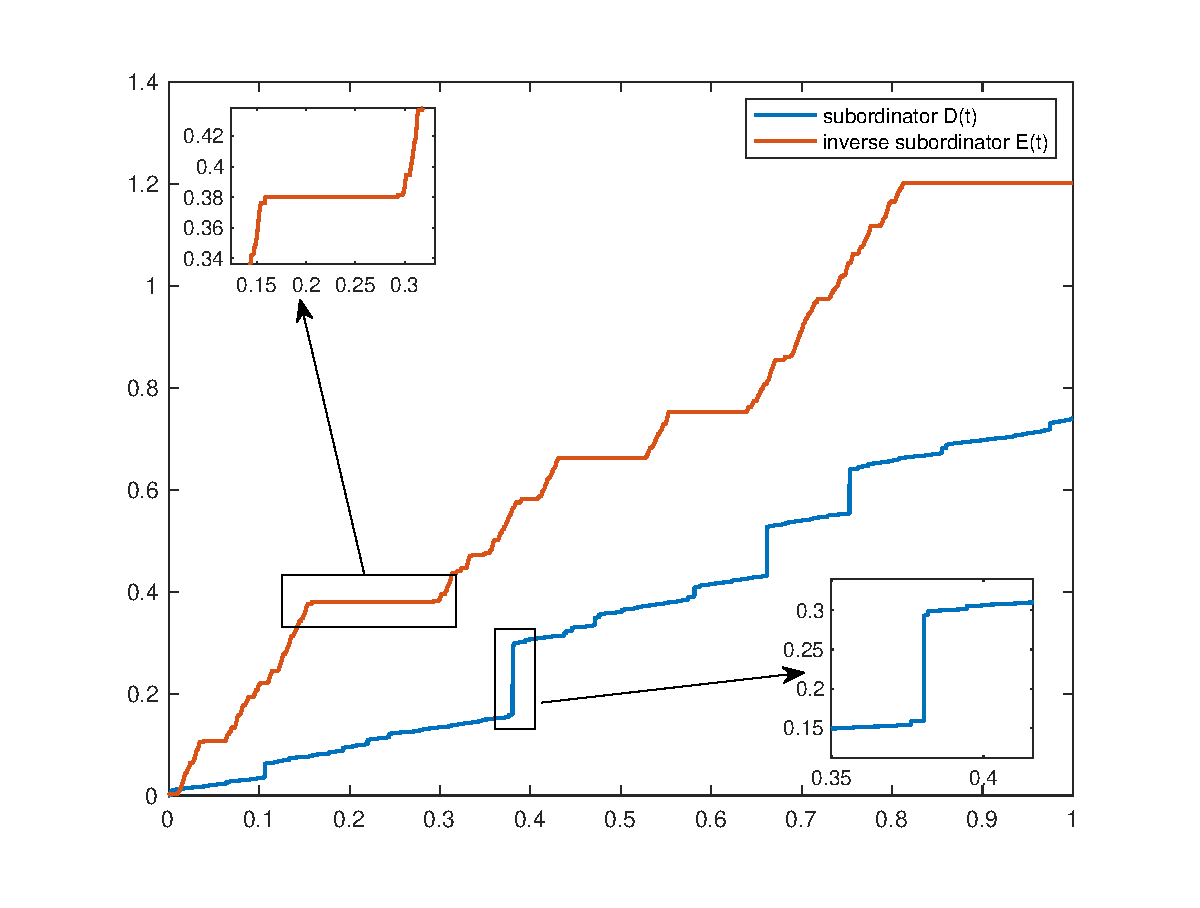
\includegraphics[width=0.45\linewidth]{DE.eps}
	\hfill
	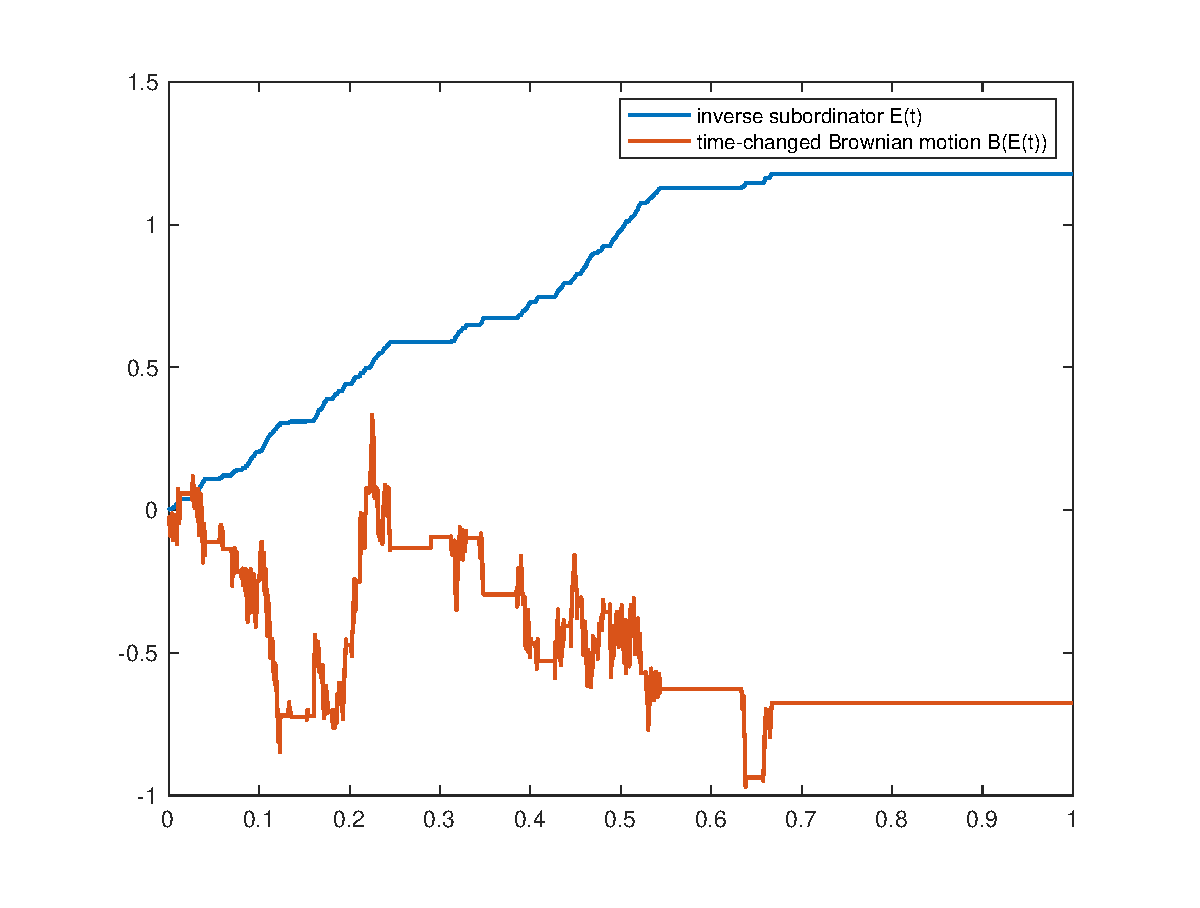
\includegraphics[width=0.45\linewidth]{BE.eps}
	\caption{左图是稳定指数$\alpha=0.8$的从属D和相应的逆从属E,右图是是稳定指数$\alpha=0.8$的逆从属E和相应的时间变换布朗运动}
	\label{fig:image1}
	\vspace{-2ex}
\end{figure}

\( E \) 和 \( B \circ E \) 都从 0 开始,对于二次变差,满足$
[B \circ E, B \circ E] = E  \text{和} [E, E] = [B \circ E, E] = 0.$
有关更一般的时间变换半鞅的随机微积分的详细信息,请参见\cite{kobayashi2011stochastic}的第 4 节。

现在我们来介绍关于时间变换的Lamperti变换. 
令 $S=(l,r)$, 其中 $-\infty\leq l<r\leq\infty$,函数 $a,b$是$S\to S$ 的连续可微函数. 考虑下面的SDE:
\begin{equation}\label{original SDE}
	dy(t)=a(y(t))dE(t)+b(y(t))dB(E(t))
\end{equation}
并且假设它在S中有唯一强解,即
$$\mathbb{P}(y(t)\in S,\:t\geq0)=1.$$
如果 $b(x)>0$ 对所有的 $x\in S$都成立, 那么我们可以使用Lamperti变换
\begin{equation}\label{Lamperti}
	F(x)=\lambda\int^x\frac1{b(y)}dy
\end{equation}
对于某些$\lambda>0.$并且$F^{-1}:F(S)\to S$ 是被良好定义的, 令$x(t)=F(y(t))$利用\cite{umarov2018beyond}中的时间变换It\^{o}公式可以得到:
\begin{equation}\label{basic SDE}
	dx(t)=f(x(t))dE(t) + \lambda dB(E(t)) 
\end{equation}

其中
$$f(x)=\lambda\left(\frac{a(F^{-1}(x))}{b(F^{-1}(x))}-\frac12b^{\prime}(F^{-1}(x))\right),\quad x\in F(S),$$
$F(D)=(F(l),F(r)).$ 这种变换可以将扩散项的非线性项转换到漂移项中, 在文章后续部分, 我们将着重研究具有加性噪声的SDE\cref{basic SDE}.

\section{主要引理}

%\begin{assumption}\label{deltaE}
%	假设存在一些常数$C_k$, 使得对于任意的$s<t$都有
%	\begin{equation}
%		E(t) - E(s) \le C_k(t-s),\:a.s.
%	\end{equation}
%\end{assumption}

从\cite{umarov2018beyond}引入下面的三个关于时间变换的引理
\begin{lemma}[第一变量变换公式]\label{first}
	令 B 是一维标准的布朗运动.
	如果 $H \in L(B(t), \mathcal{F}_t)$,则 $H_{E(t-)} \in L(B_{E(t)}, \mathcal{F}_{E_t})$.
	此外,对于所有 $t \geqslant 0$,几乎处处有
	$$
	\int_0^{E_t} H_s dB(s) = \int_0^t H_{E(s-)} dB_{E(s)}.
	$$
\end{lemma}
\begin{lemma}[第二变量变换公式]\label{second}
	令 B 是一维标准的布朗运动,设 $D$ 和 $E$ 是满足 $[D \longrightarrow E]$ 或 $[D \longleftarrow E]$ 的.
	假设 $B$ 与 $E$ 同步.如果 $K \in L(B_{E(t)}, \mathcal{F}_{E_t})$,则 $(K_{D(t-)}) \in L(B(t), \mathcal{F}_{E(D_t)})$.
	此外,对于所有 $t \geqslant 0$,几乎处处有
	$$
	\int_0^t K_s dB_{E(s)} = \int_0^{E_t} K_{D(s-)} dB(s).
	$$
\end{lemma}

\begin{lemma}[It\^{o}公式]\label{ito}
	令 B 是一维标准的布朗运动. 令 $D$ 和 $E$ 满足 $[  D\longrightarrow E ]$ 或 $[  D\longrightarrow E ] .$ X是由下述SDE定义的随机过程:
	$$X(t):=\int_0^tA(s)ds+\int_0^tF(s)dE(s)+\int_0^tG(s)dB(E(s))$$
	其中 $A(s)\in$ $L( t, \mathcal{F} _{E(t)})$, $F(s)\in$ $L( E(t), \mathcal{F} _{E(t)})$, 以及 $G(s)\in$ $L( B(E(s)), \mathcal{F} _{E(t)}) .$ 如果 $f\in$ $C^2( \mathbb{R} )$, 那么
	$f(X(t))$ 是 $\mathcal{F}_{E(t)}$-半鞅, 对于所有的t $\ge$ 0,都有
	$$\begin{aligned}
		&f(X(t))-f(0)=\int_{0}^{t}f^{\prime}(X(s))A(s)ds+\int_{0}^{E(t)}f^{\prime}\left(X(D(s-))\right)F(D(s-))ds\\
		&+\int_{0}^{E(t)}f^{\prime}\big(X(D(s-))\big)G(D(s-))dB(s)+\frac{1}{2}\int_{0}^{E(t)}f^{\prime\prime}\big(X(D(s-))\big)\big\{G(D(s-))\big\}^{2}ds.
	\end{aligned}$$
\end{lemma}

下面引入离散型Gronwall不等式, 
\begin{lemma}\label{gronwall}
	令$\Delta t > 0,g_n,\lambda _n \in \mathbb{R},\eta > 0,a_1=0$,再假设$1-\eta \Delta E_j > 0$,$1 + \lambda _n > 0,n \in \mathbb{N}$,那么如果
	\begin{equation*}
		a_{n+1} \leq a_n(1+\lambda _n)+\eta a_{n+1}\Delta E_n +g_{n+1}
	\end{equation*}
	则下面的不等式成立:
	\begin{equation}
		a_n \leq \sum\limits_{j=0}^{n-1}\prod_{i=j}^{n}(1-\eta\Delta E_i)g_{j+1}\prod\limits_{l=j+1}^{n-1}(1+\lambda _l)
	\end{equation}
\end{lemma}

下面的引理对于证明本文主要定理起着关键性的作用.

引用\cite{nane2016stability}中的引理。

\begin{lemma}\label{slowerthant}
	假设在逆从属过程$E(t)$的Laplace变换中, $\psi(s)=s^{\alpha}$, 那么
	\begin{equation}
	\lim_{t\to\infty}\frac{E_t}{t}=0,\:a.s.
	\end{equation}
\end{lemma}


\begin{lemma}
	
		如果 $E$ 是从属过程 $D$ 的逆,其拉普拉斯指数 $\psi$ 在无穷大处的正则变化指数是 $\beta \in [0, 1)$ 。如果 $\beta = 0$,进一步假设 $\nu(0, \infty) = \infty$。固定 $\lambda > 0$, $t > 0$ 和 $r > 0$。
		\begin{enumerate}
			\item[(1)] 如果 $r < \frac{1}{1 - \beta}$,则 $\mathbb{E}\left[ e^{\lambda E_t^r} \right] < \infty$。
			\item[(2)] 如果 $r > \frac{1}{1 - \beta}$,则 $\mathbb{E}\left[ e^{\lambda E_t^r} \right] = \infty$。
		\end{enumerate}
	
	
\end{lemma}



\begin{lemma}\label{main lemma}
	对于任意给定的$0 = t_0 < ih < t_1 < t_2 < \ldots <t_n <(i+1)h$,都有:
	\begin{equation}
		\mathbb{E}\left[\int_{ih}^{(i+1)h}
		\int_{ih}^{t_n} \ldots \int_{ih}^{t_2} 1 dE(t_1) \ldots dE(t_{n-1})dE(t_n)\right] \le Ch^{1+(n-1)\beta}
	\end{equation}
	,其中C是与$h$无关的常数.
\end{lemma}


\begin{proof}    
	现在,在 $[0, \infty)$ 上引入随机测度 $\Pi$,定义为 $\Pi((s, t]) = E(t) - E(s)$,其中 $t > s \geq 0$.令 $\{C(t)\}_{t \geq 0}$ 为由 $\Pi$ 驱动的Cox过程,即在条件 $\Pi = \lambda$ 下,$\{C(t)\}$ 的分布与强度为 $\lambda$ 的非齐次泊松过程等价.注意,根据\cite{kingman1964doubly},$\{C(t)\}$ 是具有更新函数的更新过程:
	\begin{equation}
		u(t) = \mathbb{E}[C(t)] = \mathbb{E}[E(t)] = \frac{t^\alpha}{\Gamma(\alpha+1)}
	\end{equation}
	对于更新过程$C(t)$,参见\cite{daley2003introduction},可以得到
	\begin{equation*}
		\mathbb{E}[\mathrm{d}C(t_n)\ldots\mathrm{d}C(t_1)] = \prod_{i=1}^n u^{\prime}(t_i - t_{i-1})\mathrm{d}t_i
	\end{equation*}
	其中$0 = t_0 < t_1 < t_2 < \ldots <t_n$. 由于 Cox 过程$C(t)$的阶乘矩等于其驱动测度$\Pi$的普通矩,参见\cite{daley2003introduction}我们得到
	\begin{equation*}
		\mathbb{E}[\mathrm dE(t_n)\ldots\mathrm dE(t_1)]=\prod_{i=1}^nu'(t_i-t_{i-1})\mathrm dt_i.
	\end{equation*}
	因此:
	\begin{align*}
		I &= \mathbb{E}\left[\int_{ih}^{(i+1)h}
		\int_{ih}^{t_n}\int_{ih}^{t_{n-1}} \ldots \int_{ih}^{t_{2}} 1 dE(t_1) \ldots dE(t_{n-2})dE(t_{n-1})dE(t_n)\right] \\
		& = \int_{ih}^{(i+1)h}\int_{ih}^{t_n}\int_{ih}^{t_{n-1}}
		\ldots \int_{ih}^{t_{2}} 1 \mathbb{E}\left[dE(t_1) \ldots dE(t_{n-2})dE(t_{n-1})dE(t_n)\right] \\
		& = \frac{\alpha^n}{\Gamma^n(\alpha+1)}
		\int_{ih}^{(i+1)h}\int_{ih}^{t_n}\int_{ih}^{t_{n-1}} \ldots \int_{ih}^{t_{2}} \prod_{i=1}^{i=n}(t_i-t_{i-1})^{\alpha -1} dt_1 \ldots dt_{n-1}dt_n
	\end{align*}
	下面单独考虑积分项:
	\begin{equation*}
		I_{1}=\int_{ih}^{t_{2}} (t_{2}-t_1)^{\alpha -1} t_1^{\alpha - 1} dt_1 \\
	\end{equation*}
	做如下变换,令$t_{1} = ih + s_{1}h$,同时$t_2 = ih + s_2h ,$,其中$h$是步长,因此$s_1,s_{2} \in [0,1]$,注意由于我们不考虑时间在原点处,因此这里的$i=\frac{T}{h}$,这里的$T$是一个时间范围,于是
	\begin{align*}
		I_1 &= \int_{0}^{s_{2}} (s_{2}-s_{1})^{\alpha -1}h^{\alpha -1} (ih + s_1h)^{\alpha - 1}h ds_1 \\
		&= h^{\alpha}\int_{0}^{s_{2}} (s_{2}-s_{1})^{\alpha -1} (ih + s_1h)^{\alpha - 1} ds_1
	\end{align*}
	由于$(ih + s_1h)^{\alpha - 1}$关于$s_1$在$[0,1]$是单调递减的,并且积分$I_n$中,被积函数和积分区域都是正的,因此
	\begin{align*}
		I_1 &\le h^{\alpha}\int_{0}^{s_{2}} (s_{2}-s_{1})^{\alpha -1} (ih)^{\alpha - 1} ds_1 \\
		&=  T^{\alpha - 1}h^{\alpha}\int_{0}^{s_{2}} (s_{2}-s_{1})^{\alpha -1} ds_1
	\end{align*}
	令$w_1=s_{2}-s_{1}$,于是
	\begin{equation*}
		I_1\le T^{\alpha - 1}h^{\alpha}\int_{0}^{s_{2}} (s_{2}-s_{1})^{\alpha -1} ds_1
		=  T^{\alpha - 1}h^{\alpha}\int_{0}^{s_{n2}} w_1^{\alpha -1} dw_1
		=  \frac{T^{\alpha - 1}s_{2}^\alpha}{\alpha}h^{\alpha}
	\end{equation*}
	因此:
	\begin{equation*}
		I \le Ch^\alpha
		\int_{ih}^{(i+1)h}\int_{ih}^{t_n}\int_{ih}^{t_{n-1}} \ldots \int_{ih}^{t_{3}} 
		\prod_{i=3}^{n}(t_i-t_{i-1})^{\alpha -1} dt_{2} \ldots dt_{n-1}dt_n
	\end{equation*}
	同理,分析如下积分:
	\begin{equation*}
		I_{2} = \int_{ih}^{t_{3}}(t_{3}-t_{2})^{\alpha -1}
		dt_{2} \le Ch^\alpha 
	\end{equation*}
	因此:
	\begin{equation*}
		I \le Ch^{2\alpha}
		\int_{ih}^{(i+1)h}\int_{ih}^{t_n}\int_{ih}^{t_{n-1}} \ldots \int_{ih}^{t_{4}} 
		\prod_{i=4}^{n}(t_i-t_{i-1})^{\alpha -1} dt_{3} \ldots dt_{n-1}dt_n
	\end{equation*}
	如此进行迭代,我们得到:
	\begin{equation*}
		I \le Ch^{(n-1)\alpha}\int_{ih}^{(i+1)h} 1 dt_1 \le Ch^{1+(n-1)\alpha}
	\end{equation*}
\end{proof}

